\section{QUY TRÌNH KHAI PHÁ DỮ LIỆU}

\subsection{Mô hình tổng quan}
Quy trình chuẩn thường đi qua các bước sau: \\
Làm sạch dữ liệu $\rightarrow$ Tích hợp dữ liệu $\rightarrow$ Trích chọn dữ liệu $\rightarrow$ Chuyển đổi dữ liệu $\rightarrow$ Khai phá dữ liệu $\rightarrow$ Đánh giá mẫu $\rightarrow$ Biểu diễn tri thức.

\vfill
\begin{figure}[H]
    \centering
    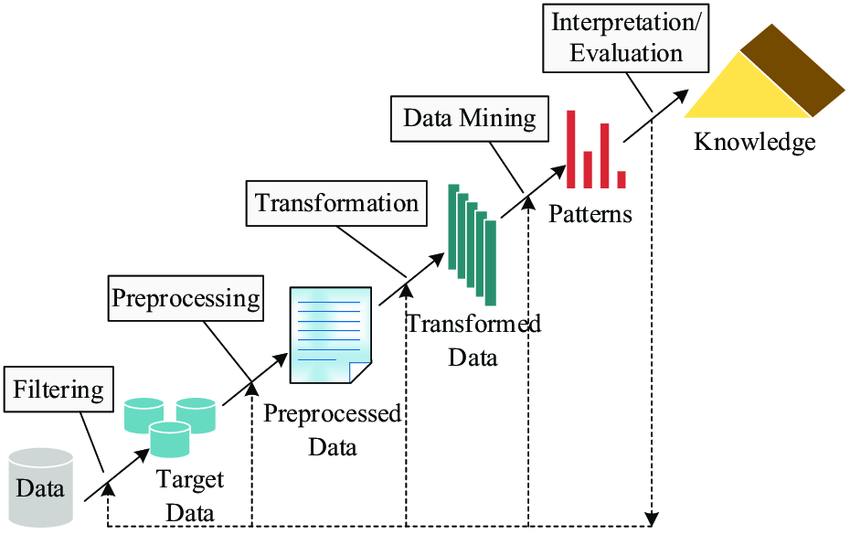
\includegraphics[width=0.65\textwidth]
    {figures/Data-mining-general-process.png}
    \caption{Sơ đồ quy trình KDD/Data Mining}
    \label{fig:data-mining-process}
\end{figure}
\clearpage

\subsection{Nhiệm vụ chi tiết từng bước}
\begin{enumerate}
    \item Làm sạch dữ liệu: Xử lý dữ liệu nhiễu, thiếu, sai sót.\\
    \textit{Ví dụ:} Điền giá trị trung bình vào các ô trống trong cột ``Tuổi''.

    \item Tích hợp dữ liệu: Hợp nhất dữ liệu từ nhiều nguồn khác nhau. \\
    \textit{Ví dụ:} Gộp bảng thông tin khách hàng và bảng lịch sử giao dịch.

    \item Trích chọn dữ liệu: Lấy ra tập dữ liệu con liên quan trực tiếp đến mục tiêu phân tích. \\
    \textit{Ví dụ:} Chỉ lấy dữ liệu khách hàng tại TP.HCM trong năm 2024.

    \item Chuyển đổi dữ liệu: Biến đổi dữ liệu về định dạng phù hợp cho thuật toán. \\
    \textit{Ví dụ:} Chuẩn hóa dữ liệu lương về đoạn $[0,1]$.

    \item Khai phá dữ liệu: Áp dụng các thuật toán thông minh để tìm mẫu. \\
    \textit{Ví dụ:} Dùng thuật toán Apriori tìm luật kết hợp, KNN để phân lớp.

    \item Đánh giá mẫu: Kiểm tra độ tin cậy và ý nghĩa của các mẫu tìm được.\\
    \textit{Ví dụ:} Loại bỏ các luật có độ tin cậy thấp, giữ lại luật giá trị.

    \item Biểu diễn tri thức: Trình bày kết quả cho người dùng cuối.\\
    \textit{Ví dụ:} Vẽ biểu đồ, bảng biểu, báo cáo trực quan.
\end{enumerate}

\subsection{Tiền xử lý dữ liệu và Trích xuất đặc trưng}
\textbf{Mục tiêu:} Giải quyết các vấn đề của dữ liệu thô như thiếu, nhiễu, trùng lặp, không nhất quán và quá nhiều chiều dữ liệu.

\subsubsection*{a. Tiền xử lý dữ liệu}
\begin{itemize}
    \item Feature Extraction: Tạo ra các đặc trưng có ý nghĩa từ dữ liệu thô.
    \item Feature Selection: Chọn lọc các đặc trưng quan trọng nhất ($k$ đặc trưng từ $n$ đặc trưng ban đầu), loại bỏ thông tin dư thừa.
    \item Feature Reduction: Giảm số chiều dữ liệu bằng cách biến đổi hoặc kết hợp đặc trưng.
    \item Normalization: Đưa các đặc trưng về cùng một khoảng giá trị (Min-Max hoặc Z-score).
\end{itemize}

\subsubsection*{b. Chi tiết về Giảm chiều dữ liệu}
\begin{enumerate}
    \item \textbf{Feature Selection}
    \begin{itemize}
        \item Khái niệm: Chọn ra tập con $k$ đặc trưng quan trọng nhất từ $n$ đặc trưng ban đầu ($k < n$), giữ nguyên ý nghĩa vật lý gốc.
        \item Ví dụ: Bộ dữ liệu bệnh tim có 20 chỉ số $\rightarrow$ Chỉ chọn 8 chỉ số quan trọng nhất để dự đoán.
    \end{itemize}

    \item \textbf{Feature Reduction}
    \begin{itemize}
        \item Khái niệm: Tạo ra các đặc trưng mới ít hơn số lượng ban đầu bằng cách chiếu dữ liệu sang không gian mới.
        \item Phương pháp phổ biến: PCA (Principal Component Analysis), SVD (Singular Value Decomposition).
    \end{itemize}

    \item \textbf{Thuật toán PCA}
    \begin{itemize}
        \item Định nghĩa: Phép biến đổi tuyến tính trực giao đưa các đặc trưng tương quan về các thành phần chính không tương quan.
        \item Mục đích: Giữ lại nhiều phương sai dữ liệu nhất khi giảm chiều
        \item Cơ sở toán học : Ma trận dữ liệu $X$ được phân rã thành: $X = U \Sigma V^T$.
        \item Các bước thực hiện PCA: (1) Chuẩn hóa dữ liệu; (2) Tính ma trận hiệp phương sai; (3) Tính trị riêng và vectơ riêng; (4) Chọn $k$ vectơ riêng ứng với trị riêng lớn nhất; (5) Chiếu dữ liệu ban đầu sang không gian mới tạo bởi các vectơ riêng này.
    \end{itemize}
\end{enumerate}

\subsection{Thực nghiệm PCA - Exercise 3.2.1}
\label{sec:pca321}
\subsubsection{Đề bài và dữ liệu đầu vào}
Theo bài Exercise 3.2.1 trong tài liệu hướng dẫn đã cung cấp : tạo hai bộ dữ liệu \(X_1\) và \(X_2\), mỗi bộ 400 vector ba chiều thuộc hai lớp, mỗi lớp 200 mẫu. Hai lớp có cùng ma trận hiệp phương sai:
\[
S=\begin{bmatrix}0.3&1.0&1.0\\1.0&9.0&1.0\\1.0&1.0&9.0\end{bmatrix}.
\]
\begin{itemize}
\item \textbf{Bộ \(X_1\):} \(m_1=(-6,6,6)^\top\), \(m_2=(6,6,6)^\top\).
\item \textbf{Bộ \(X_2\):} \(m_1=(-2,0,0)^\top\), \(m_2=(2,0,0)^\top\).
\end{itemize}
Yêu cầu: tính PCA và \textit{explained variance ratio}; chiếu dữ liệu lên hai thành phần chính đầu tiên; vẽ sáu đồ thị \(X_{11}\! -\! X_{12}\), \(X_{11}\! -\! X_{13}\), \(X_{12}\! -\! X_{13}\), \(Y_1\! -\! Y_2\), \(Y_1\! -\! Y_3\), \(Y_2\! -\! Y_3\) cho mỗi bộ; so sánh kết quả.
\subsubsection{Quy trình tính tay về mặt nguyên lý}
\begin{enumerate}
\item Lấy ma trận \(X\in\mathbb R^{400\times3}\), trong đó mỗi hàng là một vector dữ liệu. Lấy trung bình theo cột \(\bar x\), rồi tâm hóa \(X_c=X-\mathbf{1}\bar x^\top\).
\item Tính ma trận hiệp phương sai mẫu: \(\widehat S=\frac1{399}X_c^\top X_c\).
\item Tính trị riêng \(\lambda_1\ge\lambda_2\ge\lambda_3\) và vector riêng trực chuẩn \(v_1,v_2,v_3\) của \(\widehat S\).
\item Tỷ lệ phương sai của thành phần chính thứ \(j\): \(r_j=\lambda_j/(\lambda_1+\lambda_2+\lambda_3)\).
\item Chọn \(W_2=[v_1\ v_2]\). Dữ liệu sau giảm từ 3 còn 2 chiều: \(Z=X_cW_2\in\mathbb R^{400\times2}\). Khi cần vẽ đủ ba \(Y\), tạm giữ \(Y=X_c[v_1\ v_2\ v_3]\).
\end{enumerate}
\subsubsection{Kết quả chạy mã nguồn (seed = 42)}
Để có thể tái lập, dùng NumPy \texttt{default\_rng(42)}, sinh 200 mẫu mỗi lớp theo Gaussian nhiều chiều, sau đó \texttt{sklearn.decomposition.PCA} trên toàn bộ 400 mẫu \textit{không dùng nhãn lớp}. Kết quả thực thi:
\begin{center}\small\begin{tabular}{|l|r|r|r|r|}\hline
Tập&PC1 (\%)&PC2 (\%)&PC3 (\%)&PC1+PC2 (\%)\\\hline
X1&66.78&19.66&13.56&86.44\\\hline
X2&45.68&36.10&18.22&81.78\\\hline
\end{tabular}\end{center}
\noindent\textbf{Cách diễn giải:} Ví dụ tỷ lệ của \(X_1\) ở PC1 biểu thị phần phương sai dữ liệu được giữ lại khi chỉ chiếu lên vector riêng thứ nhất. Dùng hai PC sẽ giữ tổng tỷ lệ ở cột cuối. Đó là \textit{phương sai}, không trực tiếp là accuracy phân lớp.
\subsubsection{Mã nguồn Python thực nghiệm PCA}
\lstinputlisting[language=Python,caption={Mã nguồn chạy Exercise 3.2.1: tạo dữ liệu và biểu diễn 12 scatter plot.}]{source_code/pca_ex321.py}
\subsubsection{Các biểu đồ kết quả}
\noindent\textbf{Tập X1:} Các cặp tọa độ gốc (hàng trên) và sau biến đổi PCA (hàng dưới).
\begin{figure}[H]\centering
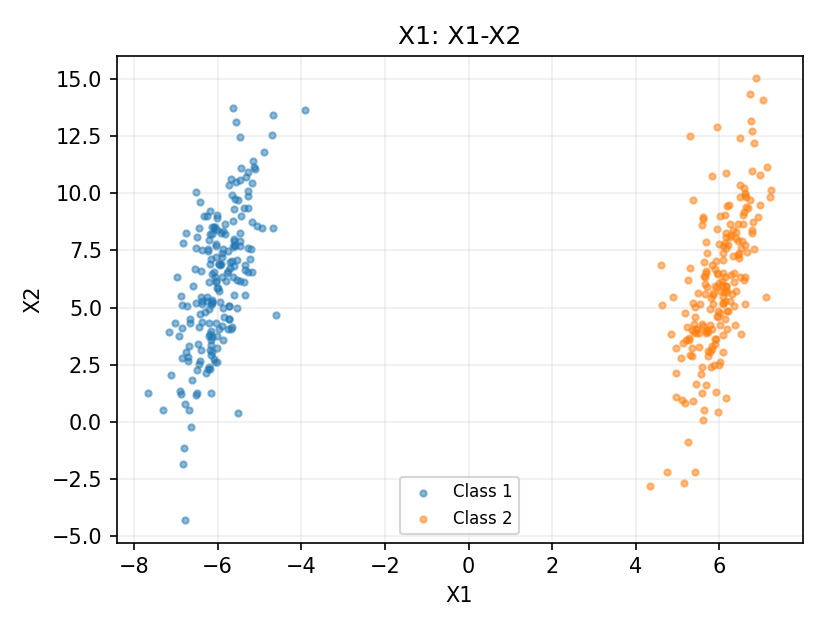
\includegraphics[width=0.315\linewidth]{figures/pca/X1_X1X2.png}\hfill
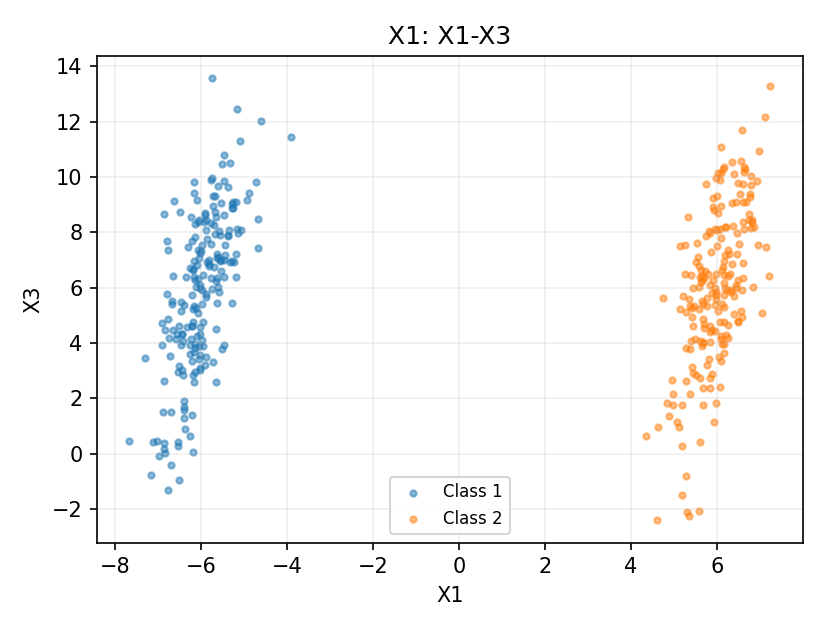
\includegraphics[width=0.315\linewidth]{figures/pca/X1_X1X3.png}\hfill
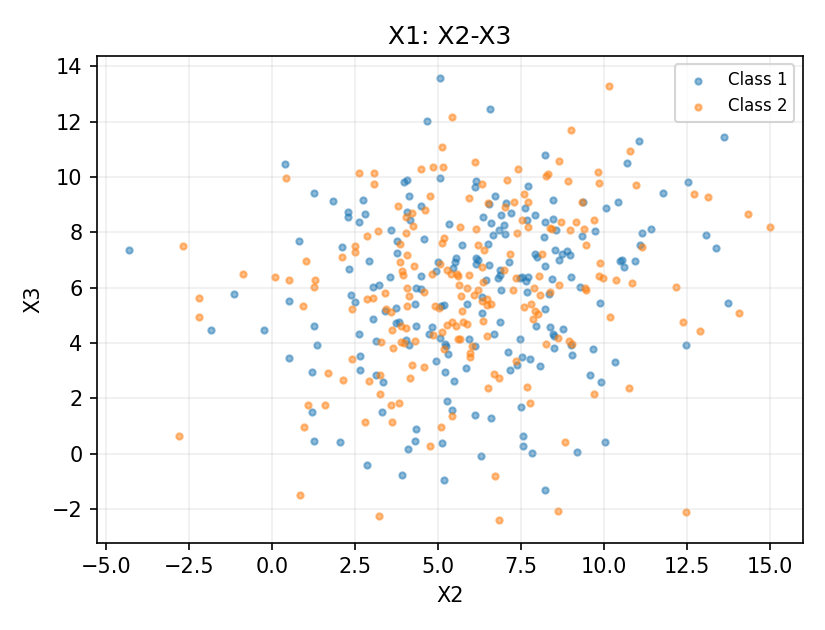
\includegraphics[width=0.315\linewidth]{figures/pca/X1_X2X3.png}\hfill
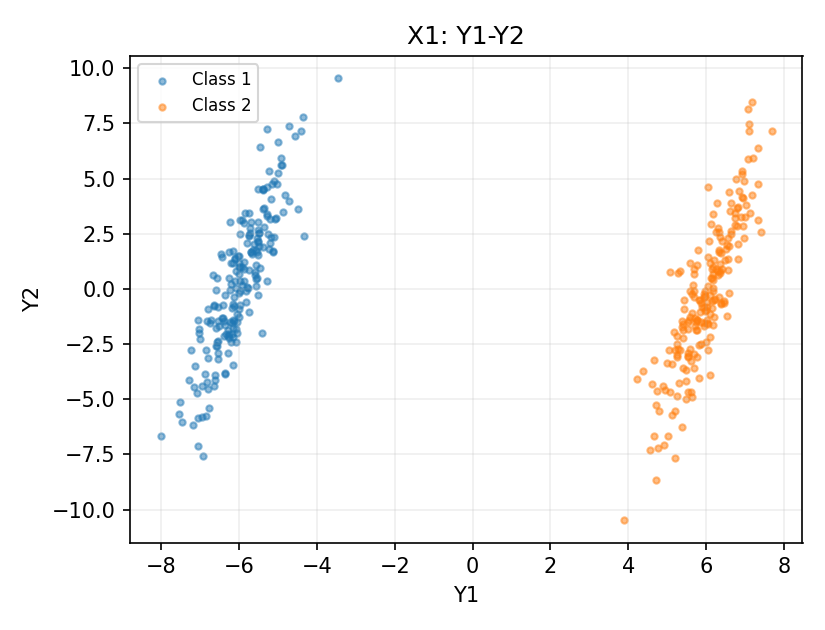
\includegraphics[width=0.315\linewidth]{figures/pca/X1_Y1Y2.png}\hfill
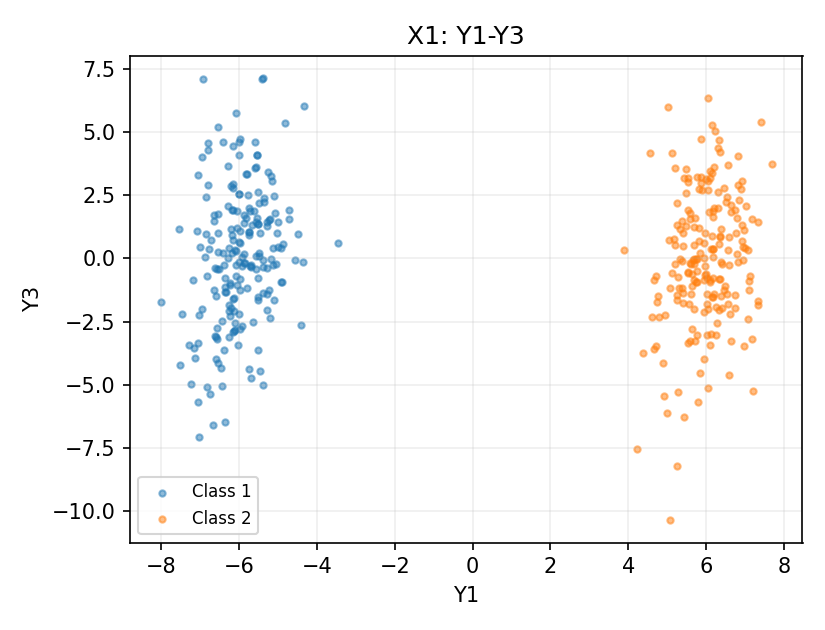
\includegraphics[width=0.315\linewidth]{figures/pca/X1_Y1Y3.png}\hfill
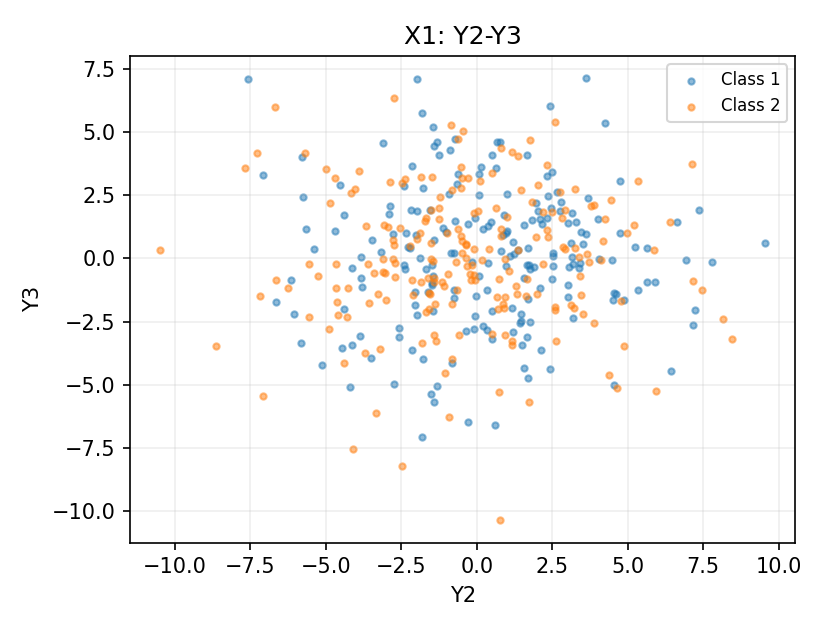
\includegraphics[width=0.315\linewidth]{figures/pca/X1_Y2Y3.png}\hfill
\caption{Sáu scatter plot của X1 theo yêu cầu Exercise 3.2.1.}
\end{figure}
\noindent\textbf{Tập X2:} Các cặp tọa độ gốc (hàng trên) và sau biến đổi PCA (hàng dưới).
\begin{figure}[H]\centering
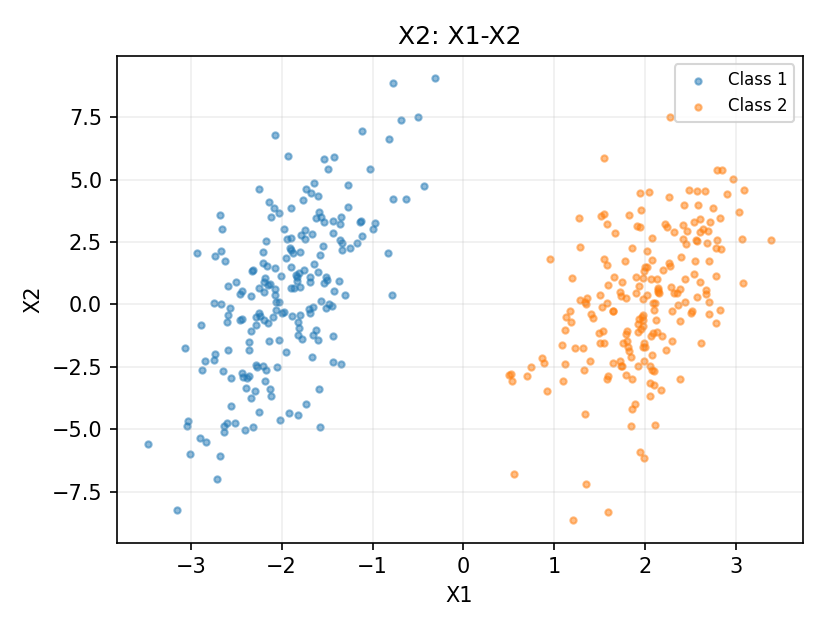
\includegraphics[width=0.315\linewidth]{figures/pca/X2_X1X2.png}\hfill
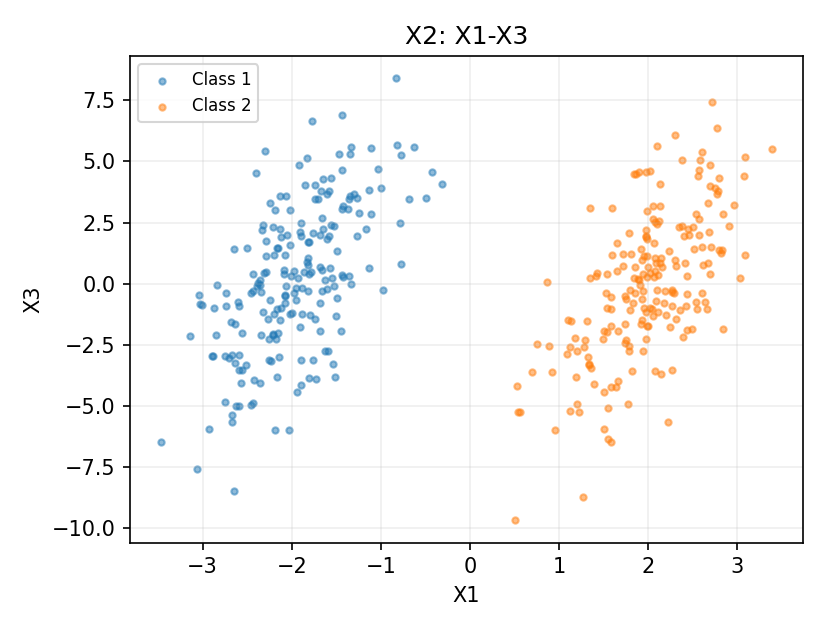
\includegraphics[width=0.315\linewidth]{figures/pca/X2_X1X3.png}\hfill
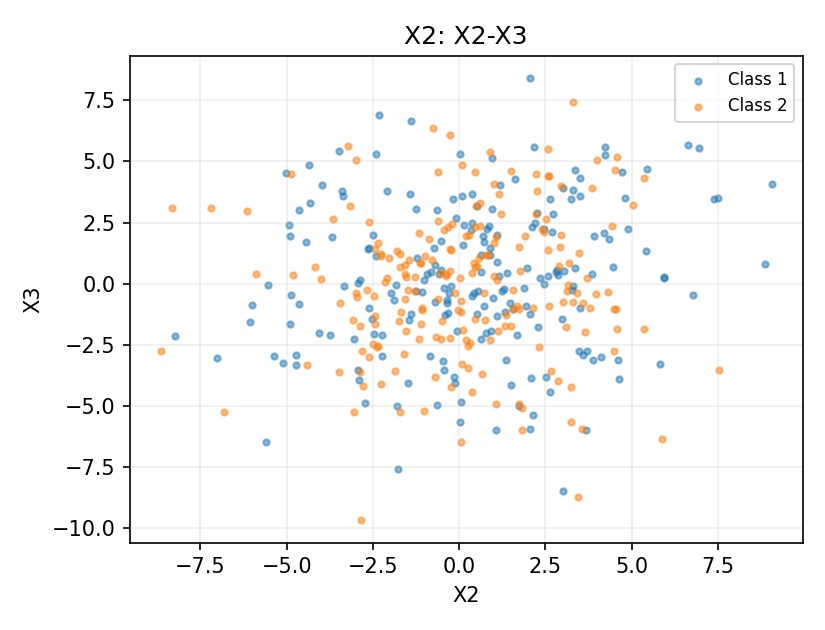
\includegraphics[width=0.315\linewidth]{figures/pca/X2_X2X3.png}\hfill
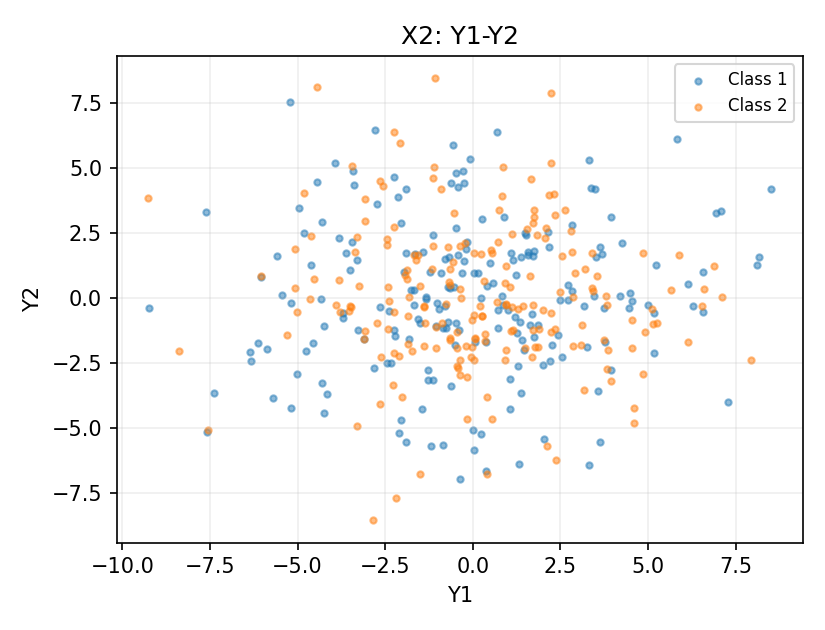
\includegraphics[width=0.315\linewidth]{figures/pca/X2_Y1Y2.png}\hfill
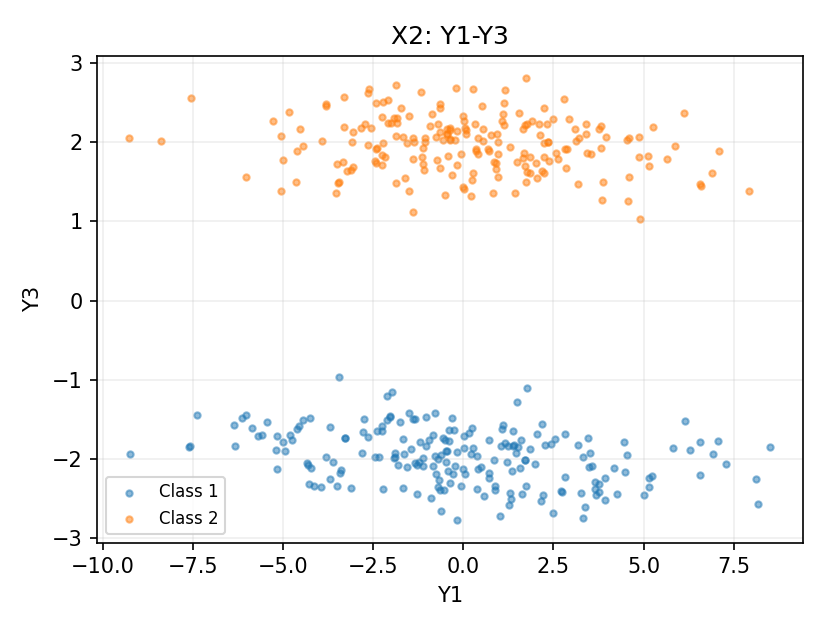
\includegraphics[width=0.315\linewidth]{figures/pca/X2_Y1Y3.png}\hfill
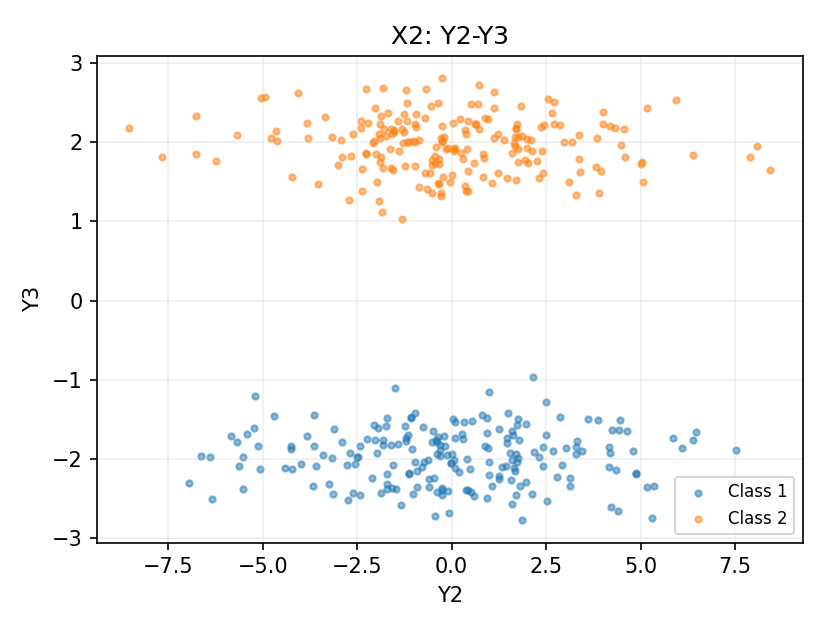
\includegraphics[width=0.315\linewidth]{figures/pca/X2_Y2Y3.png}\hfill
\caption{Sáu scatter plot của X2 theo yêu cầu Exercise 3.2.1.}
\end{figure}
\subsubsection{Nhận xét và kết luận}
\begin{itemize}
\item Ở \(X_1\), hai lớp lệch nhau rất rõ theo chiều thứ nhất, và PC1 giữ phần lớn phương sai vì còn có khác biệt trung bình giữa các lớp; giảm xuống 2 chiều vẫn thể hiện khá rõ sự tách biệt.
\item Ở \(X_2\), khoảng cách giữa hai trung bình lớp nhỏ hơn; PC1, PC2 chia sẻ phương sai tương đối đồng đều, và phép chiếu chỉ để bảo toàn phương sai không bảo đảm tối ưu khả năng phân lớp.
\item Kết quả phụ thuộc vào mẫu sinh ngẫu nhiên nên có thể khác các tỷ lệ trong ví dụ của sách; mọi số liệu ở bảng trên là kết quả chạy trực tiếp với seed 42, không sao chép từ ví dụ khác.
\end{itemize}

%\noindent\textbf{Mã nguồn tái lập:} \path{source_code/pca_ex321.py}; dữ liệu chiếu 2D xuất ra \path{figures/pca/X1_PCA_2D.csv} và \path{figures/pca/X2_PCA_2D.csv}.